\documentclass{beamer}
\usepackage{graphicx}
\usepackage{paralist}
\usepackage{outlines}

\title{Healing Brush Tool}
\author{Mendocino College - Digital Image Manipulation with Photoshop}
\titlegraphic{\vspace{-10mm}
\includegraphics[width = .9\textwidth]{images/photoshop.jpg}} 
\date{\vspace{-5em}} 


\mode <presentation>
\usetheme{Warsaw}
\usecolortheme{default}

\setbeamerfont{footline}{size=\fontsize{5}{8}\selectfont}

\definecolor{darkred}{rgb}{20,0,0}
\definecolor{darkgreen}{RGB}{40,110,20}
\definecolor{darkpurple}{RGB}{30,0,30}
\definecolor{chardonnay}{RGB}{255, 255, 204}

\setbeamercolor*{palette primary}{fg=white, bg=darkgreen}


\begin{document}
	{
		\setbeamertemplate{footline}{} 
		\setbeamertemplate{headline}{} 
		\begin{frame}
			\vspace{-35pt}
			\maketitle
		\end{frame}
	}


		\section{Spot Healing Brush Tool}
			\subsection{Spot Healing Brush Tool}		
			\begin{frame}
				\frametitle{Spot Healing Brush Tool}
				\begin{outline}
					\1 Hide unwanted items and remove small objects from a photo with this powerful retouching tool.
					\1 The Spot Healing Brush tool quickly removes blemishes and other imperfections in your photos. 
					\1 It paints with sampled pixels from an image or pattern and matches the texture, lighting, transparency, and shading of the sampled pixels to the pixels being healed. 
					\1 The Spot Healing Brush does not require you to specify a sample spot. 
					\2 It automatically samples from around the retouched area.
				\end{outline}
			
			\end{frame}
					\begin{frame}
			\frametitle{How to use the Spot Healing Brush Tool}
			\begin{outline}
				\1 First select the layer that contains spots or small objects you want to remove, In the Layers panel.
				\1 Select the Spot Healing Brush tool In the Tools panel.
				\1 Adjust the brush size and hardness of the Spot Healing Brush tool to fit the item you’re trying to remove, In the options bar.
				\1 Click on a spot or drag over an object you want to remove. 
			\end{outline}
		\end{frame}

	\subsection{Example}		
	\begin{frame}
		\frametitle{Spot Healing Example}
		\begin{center}
			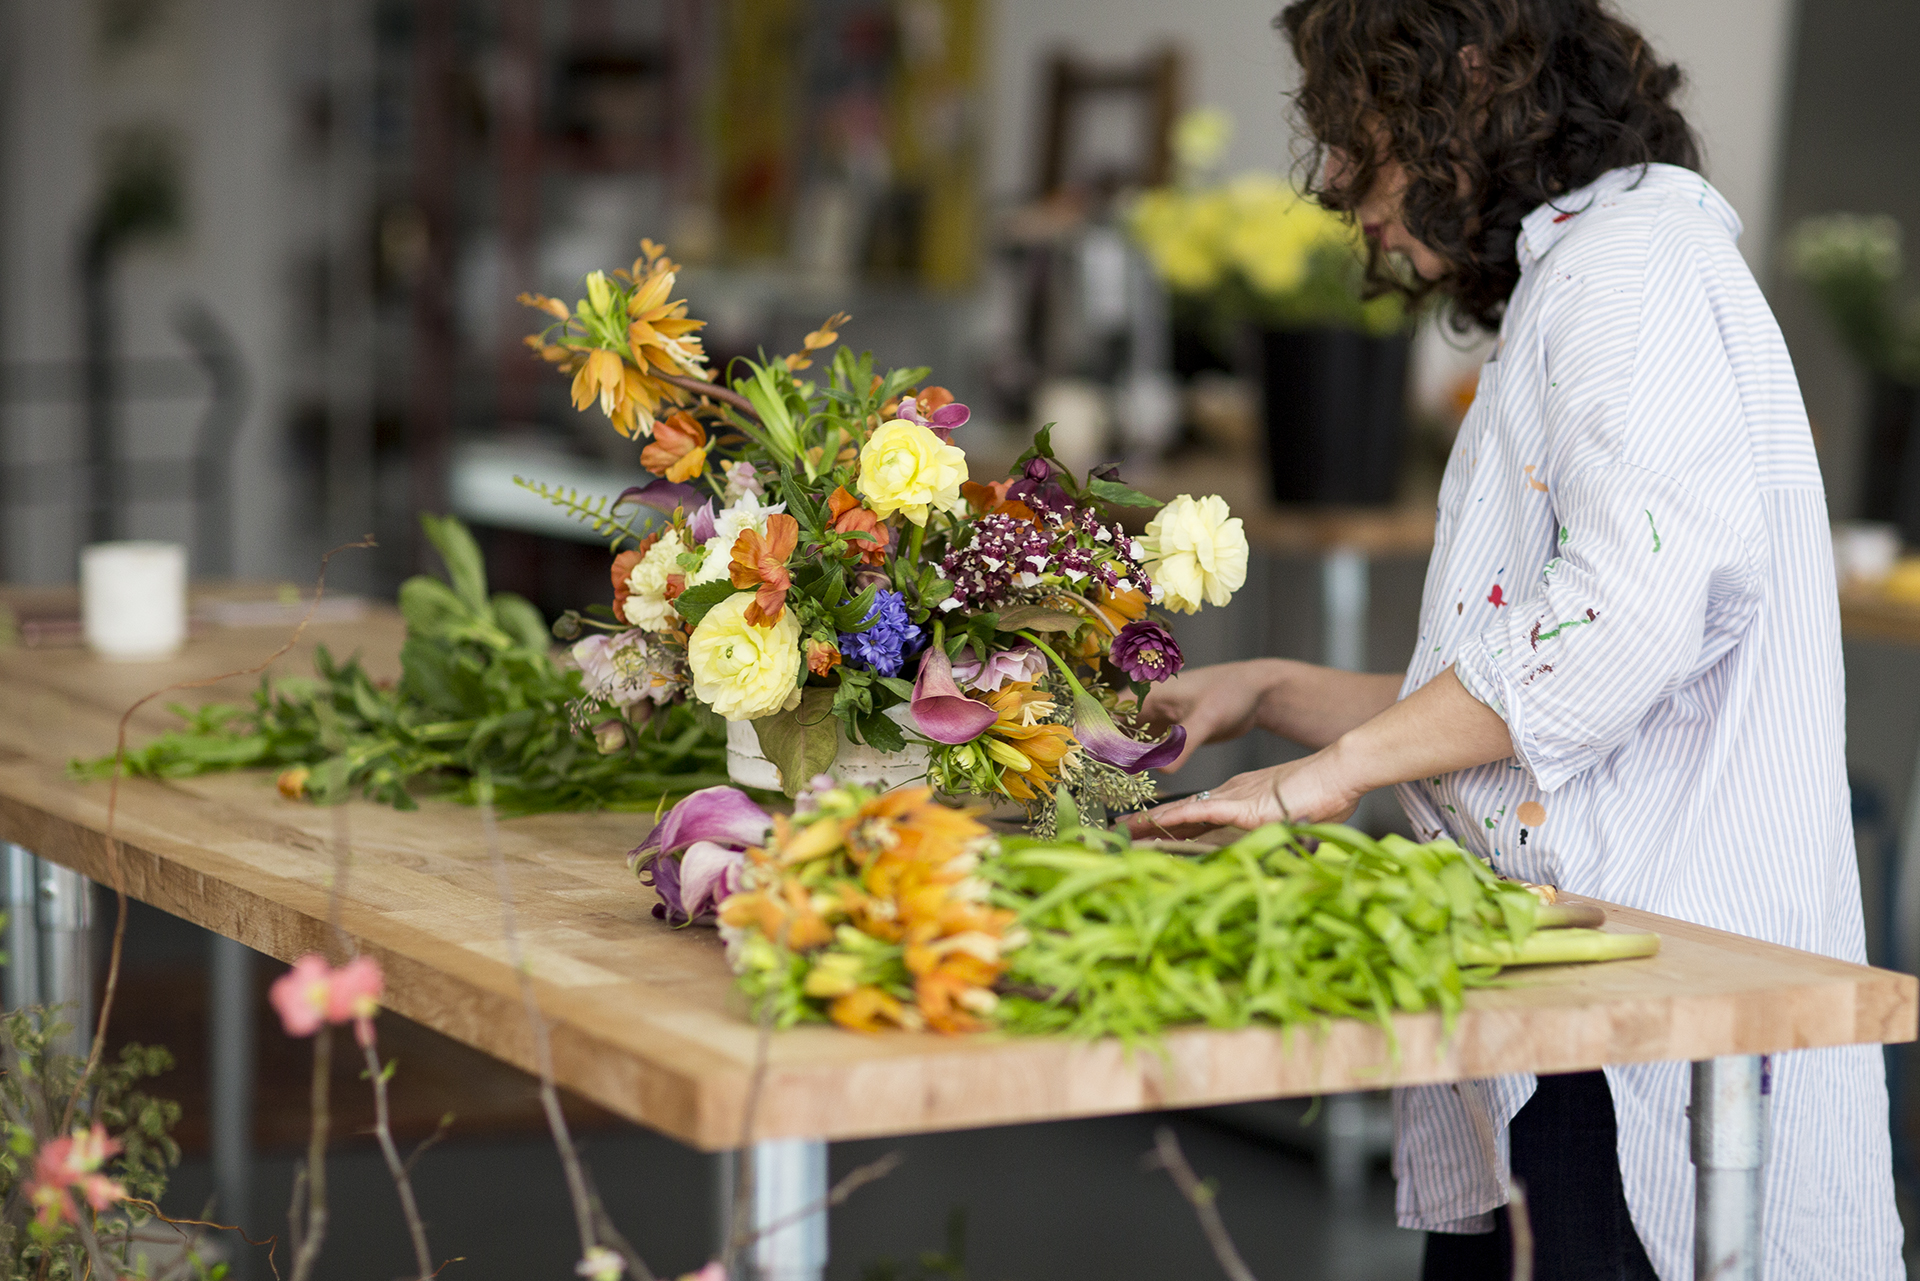
\includegraphics[width=0.890\textwidth]{images/spot-healing-brush-tool.PNG}
		\end{center}
	\end{frame}

\subsection{Options}		
\begin{frame}
	\frametitle{Spot Healing Options}
	\begin{outline}
		\1 Proximity Match - 
		\2 Uses pixels around the edge of the selection to find an area to use as a patch.
		
		\1 Create Texture - 
		\2 Uses pixels in the selection to create a texture. If the texture does not work, try dragging through the area a second time.
		
		\1 Content-Aware - 
		\2 Compares nearby image content to seamlessly fill the selection, realistically maintaining key details such as shadows and object edges.
		
		\1 Sample All Layers in the options bar to sample data from all visible layers. 
		\2 Deselect Sample All Layers to sample only from the active layer.
		
		\1 Choose a blending mode from the Mode menu in the options bar. 
		\2 Choose Replace to preserve noise, film grain, and texture at the edges of the brush stroke when using a soft‑edge brush.
	\end{outline}
\end{frame}

\subsection{Resources}		
\begin{frame}
	\frametitle{Additional Resources for the Spot Healing Brush Tool}
	\begin{outline}
		\1 How to remove objects in photoshop with spot healing brush tool
		\2 By:  Adobe
		\2 https://helpx.adobe.com/photoshop/how-to/spot-healing-brush-tool.html
	\end{outline}
\end{frame}


\section{Healing Brush Tool}
\subsection{Healing Brush Tool}		
\begin{frame}
	\frametitle{Healing Brush Tool}
	\begin{outline}
		\1 The Healing Brush tool lets you correct imperfections, causing them to disappear into the surrounding image. 
		\1 It is used for retouching large areas, and gives you more control over the sampling source.
		\1 The Healing Brush paints with sampled pixels from an image or pattern, similar to the clone stamp tool. 
		\2 However, the Healing Brush tool also matches the texture, lighting, transparency, and shading of the sampled pixels to the pixels being healed.
		\2 Resulting in the repaired pixels blending seamlessly into the rest of the image.
		\1 
	\end{outline}
\end{frame}

\begin{frame}
	\frametitle{How to use the Healing Brush Tool}
	\begin{outline}
		\1 Select the Healing Brush tool (J) from the toolbar. 
		\2 If you can’t find the Healing Brush tool, click and hold the Spot Healing Brush tool to show the other related tools, and then select the Healing Brush tool.
		\1 In the tool options bar, click the brush sample and set the brush options in the pop‑up panel — Mode, Source, Aligned, Sample, and Diffusion.
		\1 Set the source sampling area by positioning the pointer over an area in your image and Alt-click (Win) or Option-click (Mac).
		\2 You can use the Clone Source panel to select the sampled source you want to use.
		\1 Drag anywhere in the image. The sampled pixels are blended with the existing pixels each time you release the mouse button.
	\end{outline}
\end{frame}

\subsection{Example}		
\begin{frame}
	\frametitle{Healing Brush Tool Example}
	\begin{center}
	\includegraphics[width=1.0\textwidth]{images/healing brush tool.png}
	\end{center}
\end{frame}

			\subsection{Options}		
			\begin{frame}
				\frametitle{Healing Brush Tool Options}
				\begin{outline}
					\1 Mode - 
					\2 Specifies the blending mode. Choose Replace to preserve noise, film grain, and texture at the edges of the brush stroke when using a soft‑edge brush.
					
					\1 Source - 
					\2 Specifies the source to use for repairing pixels. 
					\2 Sampled to use pixels from the current image, or Pattern to use pixels from a pattern. 
					\2 If you chose Pattern, select a pattern from the Pattern pop‑up panel.
					
					\1 Aligned - 
					\2 Samples pixels continuously, without losing the current sampling point, even if you release the mouse button. 
					\2 Deselect Aligned to continue to use the sampled pixels from the initial sampling point each time you stop and resume painting.
				\end{outline}
			\end{frame}

			\begin{frame}
	\frametitle{Healing Brush Tool Options}
	\begin{outline}
		\1 Sample - 
		\2 Samples data from the layers you specify. 
		\2 To sample from the active layer and visible layers below it, choose Current And Below. 
		\2 To sample only from the active layer, choose Current Layer. 
		\2 To sample from all visible layers, choose All Layers. 
		\2 To sample from all visible layers (except adjustment layers), choose All Layers and click the Ignore Adjustment Layers icon to the right of the Sample pop‑up menu.
		
		\1 Diffusion - 
		\2 Controls how quickly the pasted region adapts to the surrounding image. 
		\2 Select a lower value for images with grain or fine details, or a higher value for smooth images.
	\end{outline}
\end{frame}
		
			\subsection{Resources}		
	\begin{frame}
		\frametitle{Additional Resource for using the Healing Brush Tool}
		\begin{outline}
			\1 How to use the Healing Brush tool in Photoshop
			\2 By:  Adobe 
			\2 https://helpx.adobe.com/photoshop/using/tool-techniques/healing-brush-tool.html
			\1 Retouch and repair photos
			\2 By:  Adobe 
			\2 https://helpx.adobe.com/photoshop/using/retouching-repairing-images.html
		\end{outline}
	\end{frame}



		\section{}
			\subsection{Destructive Edits}		
			\begin{frame}
				\frametitle{Destructive Edits}
				\begin{outline}
					\1 Applying some of these tools permanently alters the image information.
					\1 It is recommended to always work using nondestructive edits.
					\1 To edit your images non-destructively, always work on a duplicate layer. 
				\end{outline}
				\begin{center}
					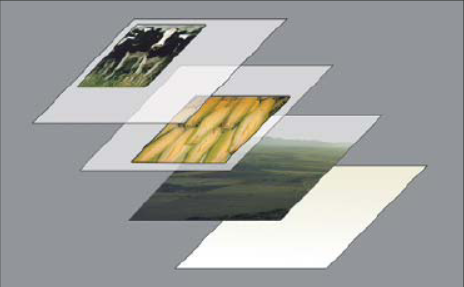
\includegraphics[width=0.7\textwidth]{images/layers example.png}
				\end{center}	
			\end{frame}
	
\end{document}